\documentclass{beamer}
\usepackage{multicol}
\usepackage{common/lstlinebgrd}
\usepackage{common/beamerthemeUpceFei}
\usepackage{common/code}

\graphicspath{{images/}} % Location of the graphics files


\newcommand\fullscreenFrameImage[2][height=\paperheight]{%
\begin{frame}[plain]
\makebox[\linewidth][c]{%
  \begin{minipage}{\dimexpr\textwidth+2cm\relax}
  \raggedright
  \colorbox{white} {
    \makebox[\linewidth]{\includegraphics[#1]{#2}}
    }        
  \end{minipage}%
  }%
  \end{frame}
}

\author{Pavel Jetenský, Petr Filip}
\title{Programování internetových aplikací}
\institute{Univerzita Pardubice}
%\date{September 18, 2007}

\newcommand{\h}[1]{H^{(1)}_{#1}}


\begin{document}



  \maketitle

 
  
\section{Organizace výuky}
  
\begin{frame}{Požadavky na studenta}
\begin{itemize}
	\item docházka -- maximálně 2 neúčasti na cvičení
	\item semestrální práce - implementace webové aplikace
	\begin{itemize}
		\item Spring boot
		\item MVC pattern
		\begin{itemize}
		  	\item Controller
			\item View - templating engine (Themyleaf/velocity/freemarker) nebo angular
			\item Model - service beans
			\item R/W of data from/to database		   
		\end{itemize}
	\end{itemize}
\end{itemize}

\end{frame}
  
  
\begin{frame}{Náplň cvičení}
	\begin{itemize}
	\item návrh a tvorba webových stránek
		\begin{itemize}
			\item  HTML + CSS - intro (Pavel)
			\item  Intro to Spring core (Pavel)
			\url {https://www.slideshare.net/PradeepReddy274/spring-core-102822350}
			\item  Testing Spring Boot Applications
			\item 
			\href{https://www.slideshare.net/SpringCentral/intro-to-spring-boot}{Intro to Spring Boot (Pavel)}
			\item  Embedding database (Pavel)\url
			{http://www.vogella.com/tutorials/SpringBoot/article.html#exercise-embedding-a-database}
			\item  CRUD - shopping cart (Petr)
			\item  Selenium/GEB Test (Pavel)
			\item  Adding REST endpoints (Petr)\url
			{http://www.vogella.com/tutorials/SpringBoot/article.html#exercise-making-the-information-available-via-rest}
			\item  Spring cloud 1 (Petr)
			\item  Spring cloud 2 (Petr)
			\item  Nasazení na server (Petr)
			\item  Common security threads and how to tackle them (Jan Novotný, Forrest)
			- úterý od 7.5. 18:00 v H1
			\item  zápočet a dodělávky (předtermín) + Konzultace 2h (Pavel) 
			\item  Další termín zkoušky + Konzultace 4h (Petr)
		\end{itemize}
\end{itemize}
\end{frame}  
  



\begin{frame}{Pracovní prostředí a nástroje I.}
	\begin{itemize}
		\item vývojové prostředí -- PHPStorm (zdarma pro studenty)
		\item webový server -- apache
		\item databázový server -- MySQL / MariaDB 
		\item webový prohlížeč -- Google Chrome
		\item verzovací systém -- GIT (github.com)
		\item modelovací nástroj pro databázi -- WorkBench	
		\item nástroj pro tvorbu diagramu - draw.io
	\end{itemize}
	
	Vše multiplatformní a zdarma!
\end{frame}

\begin{frame}{Pracovní prostředí a nástroje II.}
Vybrat jednu z následujících možností:

	\begin{itemize}
		\item Softaculous Ampps
			\begin{itemize}
				\item \url{https://youtube.com/watch?v=fH6KjaddLA0}
				\item \url{https://ampps.com/wiki/Category:Endusers}
			\end{itemize}
	\end{itemize}

	\begin{itemize}
		\item XAMPP -- \url{https://www.apachefriends.org/}
	\end{itemize}

	\begin{itemize}
		\item Docker:  \url{https://github.com/petrfilip/}
		\begin{itemize}
			\item simple-docker-web-dev-environment
			\begin{enumerate}
				\item stáhnout (přes git nebo jako zip)
				\item spustit příkaz "docker compose up"
				\item otevřít webový prohlížeč na adrese "localhost"
			\end{enumerate}
		\end{itemize}	
	\end{itemize}

\end{frame}


\begin{frame}{Marketshare - webservery}
    \makebox[\linewidth]{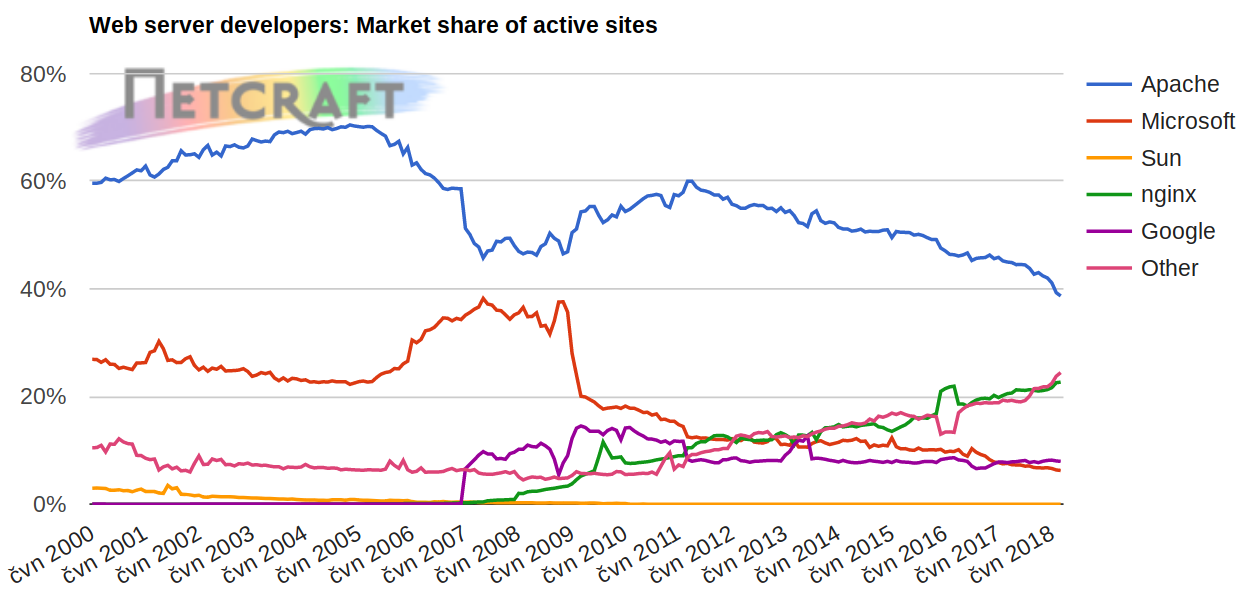
\includegraphics[width=\linewidth]{images/webserver-marketshare.png}}
\end{frame}

\begin{frame}{Marketshare - webové prohlížeče}
    \makebox[\linewidth]{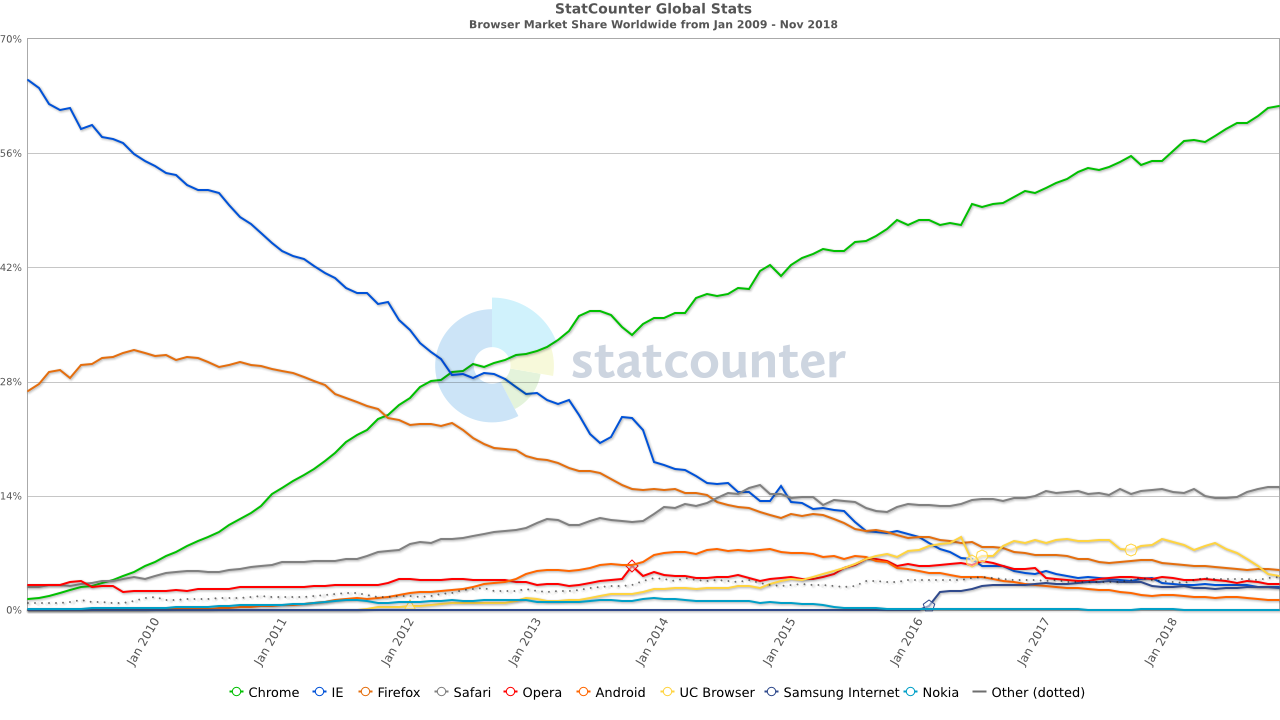
\includegraphics[width=\linewidth]{images/webbrowser-marketshare.png}}
\end{frame}

\begin{frame}{Další nástroje}

	\begin{itemize}
		\item Fakultní hosting
		\begin{itemize}
			\item https://fei-hostingadmin.upceucebny.cz/
			\item FileZilla
		\end{itemize}
	\end{itemize}

\end{frame}

\begin{frame}{Doporučené zdroje}
	\begin{itemize}
		\item https://www.w3schools.com/
	\end{itemize}
\end{frame}

\section{Jak to funguje?}

\begin{frame}[fragile, shrink=0]{Co se zobrazí v prohlížeči}
    \makebox[\linewidth]{
\includegraphics[width=\linewidth]{images/upce-screenshot.png}}
\end{frame}

\begin{frame}{Co se ve skutečnosti provede}
    \makebox[\linewidth]{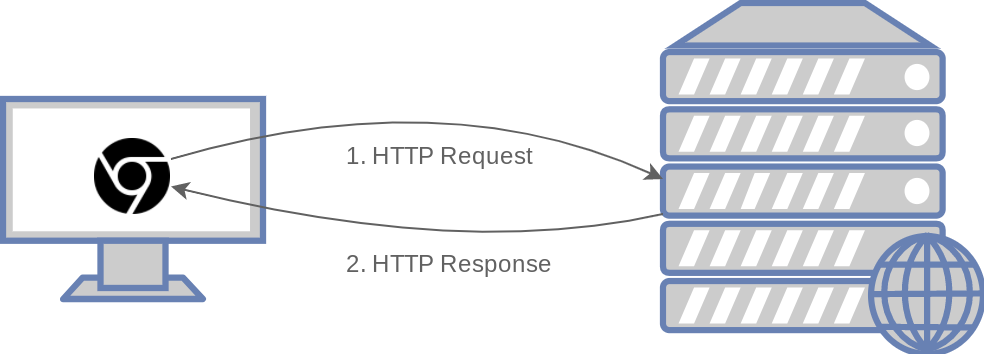
\includegraphics[width=\linewidth]{images/request-response.png}}
\end{frame}

\begin{frame}{Co vidí prohlížeč}
    \makebox[\linewidth]{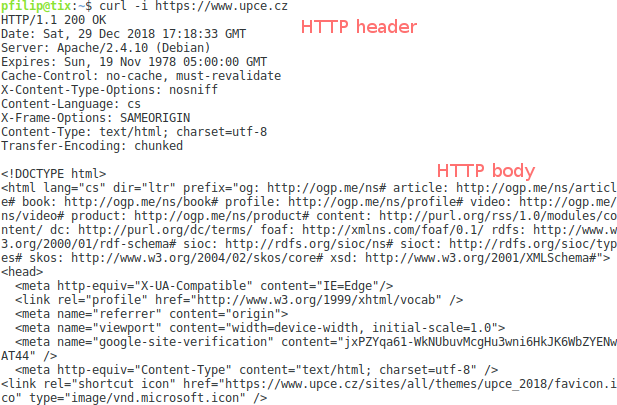
\includegraphics[width=\linewidth]{images/curl-described.png}}
\end{frame}

\begin{frame}{Z čeho se webová stránka skládá?}
  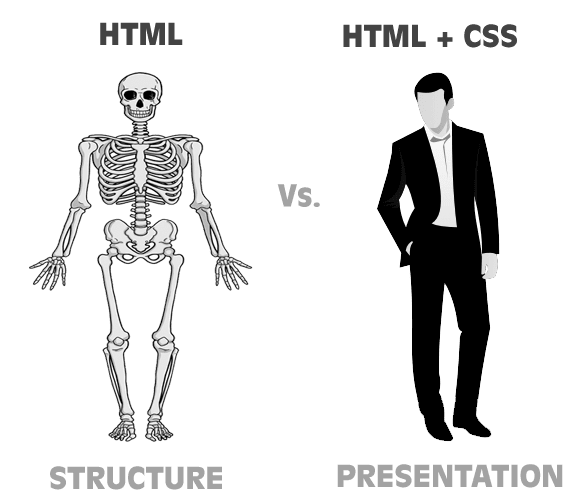
\includegraphics[width=\columnwidth]{html-vs-css}
\end{frame}

\begin{frame}[fragile, shrink=0]{Ukázka HTML kódu}

\begin{lstlisting}[language=HTML5]
<!DOCTYPE html>
<html>
  <head>
    <title>Page Title</title>
    <link rel="stylesheet" href="style.css">
  </head>
  <body>
    <h1>This is a Heading</h1>
    <p>This is a paragraph.</p>
  </body>
</html>
\end{lstlisting}

\end{frame}

\begin{frame}[fragile, shrink=0]{Ukázka CSS kódu}
\begin{itemize}
	\item style.css
\end{itemize}
\begin{lstlisting}[language=CSS]
body {
    background-color: lightblue;
}

h1 {
    color: white;
    text-align: center;
}

p {
    font-family: verdana;
    font-size: 20px;
}
\end{lstlisting}
\end{frame}


\begin{frame}{Co vše se načítá?}
    \makebox[\linewidth]{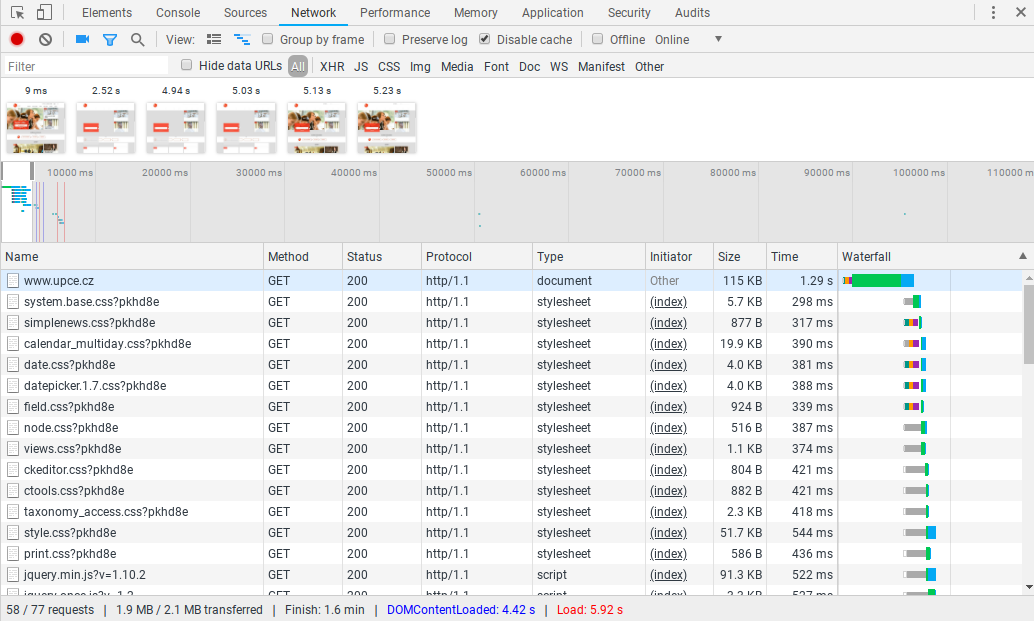
\includegraphics[width=\linewidth]{images/devtools-network.png}}
\end{frame}


\section{Projektové cvičení}

\begin{frame}{Proč dělat web?}
	\begin{itemize}
		\item Proč budu web dělat? 
		\item Komu bude sloužit?
		\item Jak si web představujete?
		\item Co má web obsahovat?
		\item dymický x statický?
		\item Jak ho vypublikuji?
	\end{itemize}
\end{frame}

\begin{frame}{Projektové cvičení - cíle}
	\begin{itemize}
		\item vytvořit eshop pro prodej licencí k softwaru
		\begin{itemize}
			\item analýza
			\begin{itemize}
				\item model businessu pro rychlé zasvěcení -> rich picture
				\item aktéři, požadavky, funkce -> use case diagram
				\item modelování procesů -> activity diagram
				\item modelování databáze -> schema diagram
			\end{itemize}
			\item implementace
			\begin{itemize}
				\item založit projekt a nastavit prostředí
				\item programovat
			\end{itemize}
			
		\end{itemize}
	\end{itemize}
\end{frame}

\begin{frame}{Projektové cvičení - technologie}
	\begin{itemize}
		\item Jak a jaké technologie zvolit?
		\item Pro náš projekt:
		\begin{itemize}
			\item HTML
			\item CSS
			\item PHP
			\item Databáze
			\item JS
		\end{itemize}
	\end{itemize}
\end{frame}

\begin{frame}{Rich picture}
	\begin{itemize}
		\item slouží ke komplexnímu pochopení celého problému/situace
		\item jednoduchý popis projektu a core businessu pomocí obrázku
		\item nejde o jazyk
	\end{itemize}

	\begin{itemize}
		\item zobrazuje aktéry, akce a základní funkce
	\end{itemize}
\end{frame}

\begin{frame}{Rich picture}
  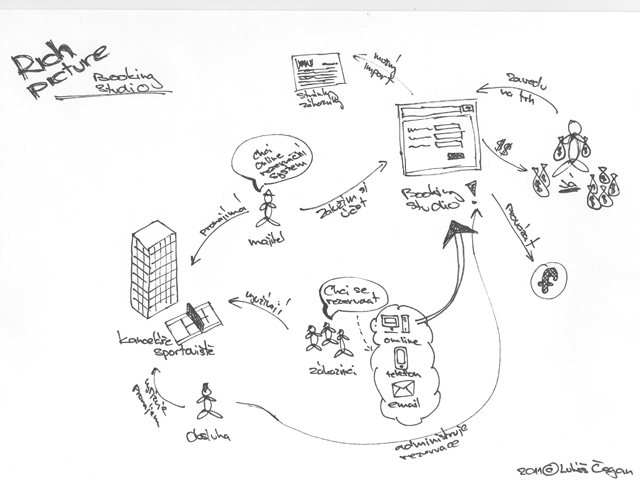
\includegraphics[width=\columnwidth]{rich-picture}
\end{frame}

\begin{frame}{Wireframe}
	  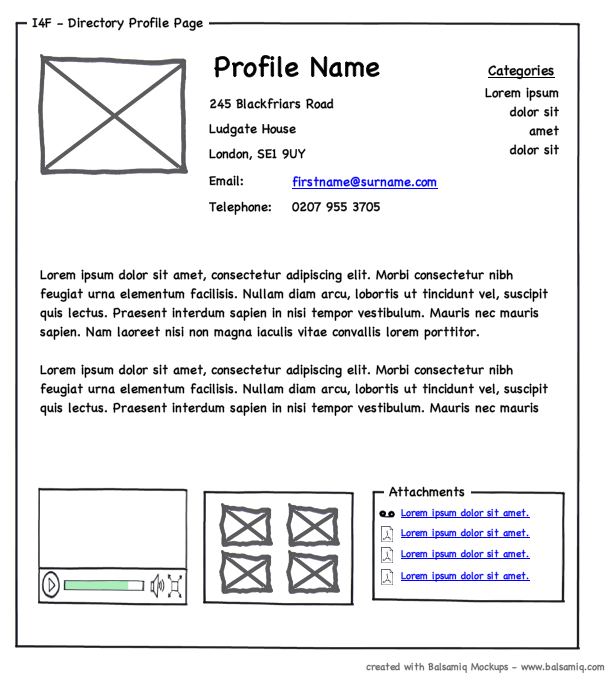
\includegraphics[width=\textwidth,height=\textheight,keepaspectratio]{wireframe}
\end{frame}

\begin{frame}{Responzivní wireframe}
	  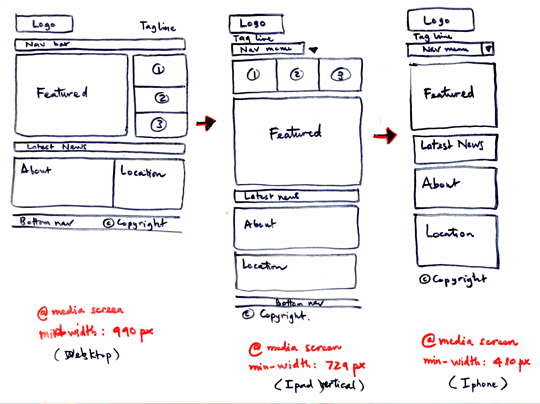
\includegraphics[width=\columnwidth]{responsive-wireframe}
\end{frame}

\begin{frame}{Mapa webu - sitemap}
	  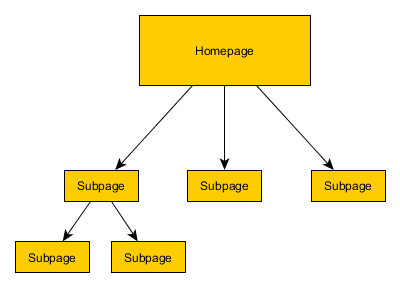
\includegraphics[width=\columnwidth]{sitemap}
\end{frame}


\begin{frame}{Storyboard}
	  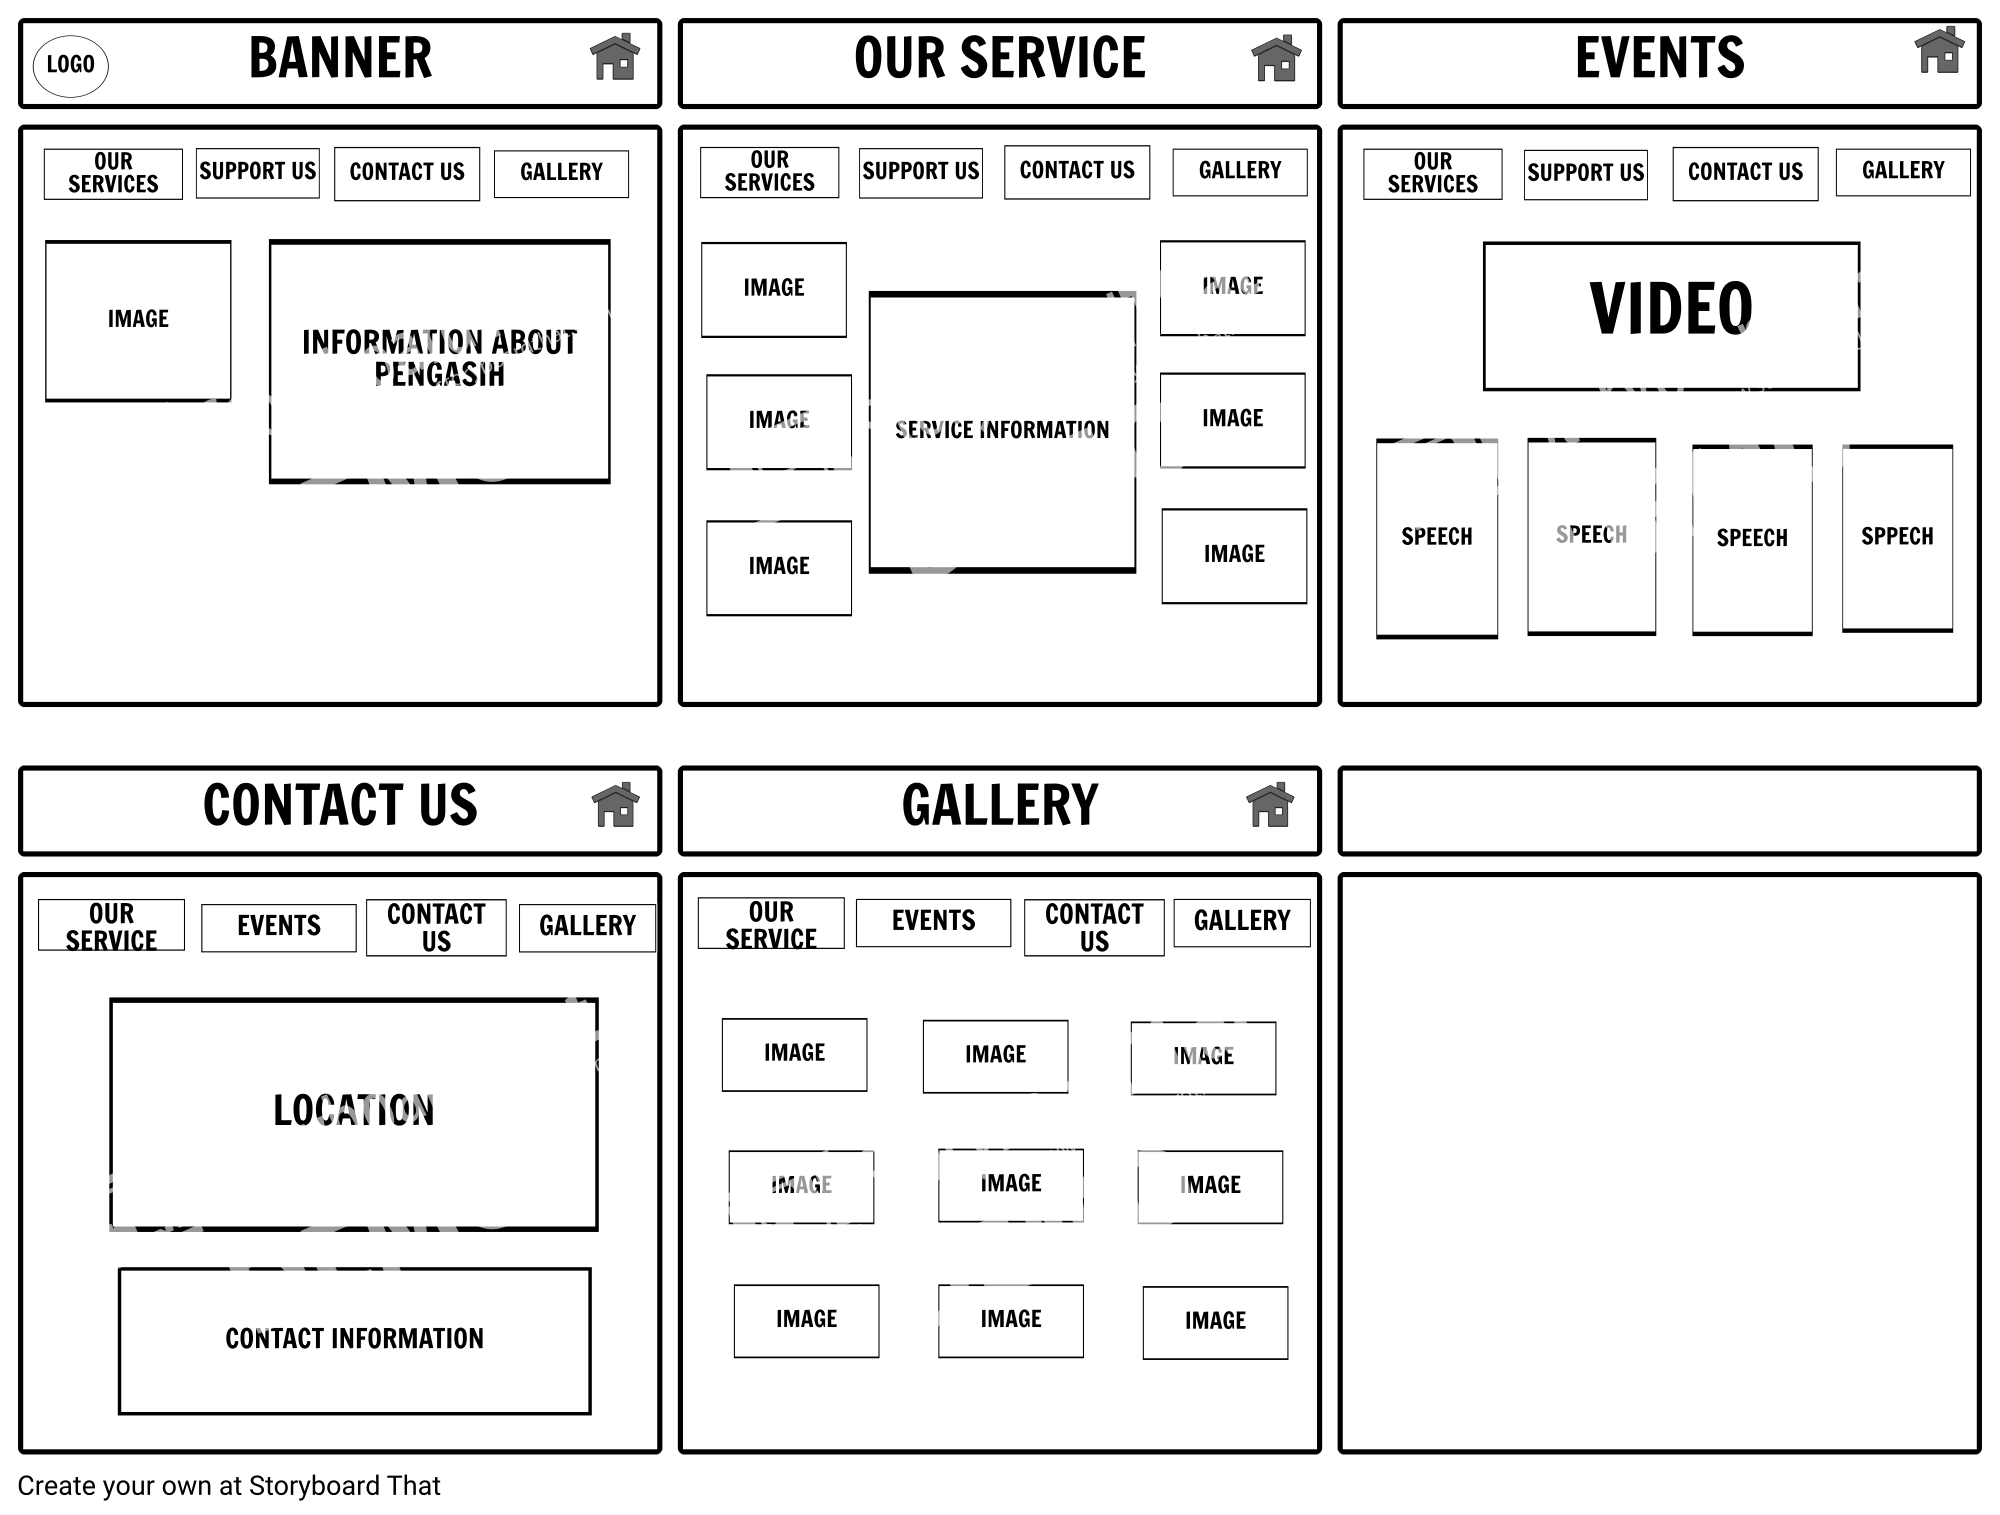
\includegraphics[width=\columnwidth]{storyboard}
\end{frame}

\begin{frame}{Storyboard}
	  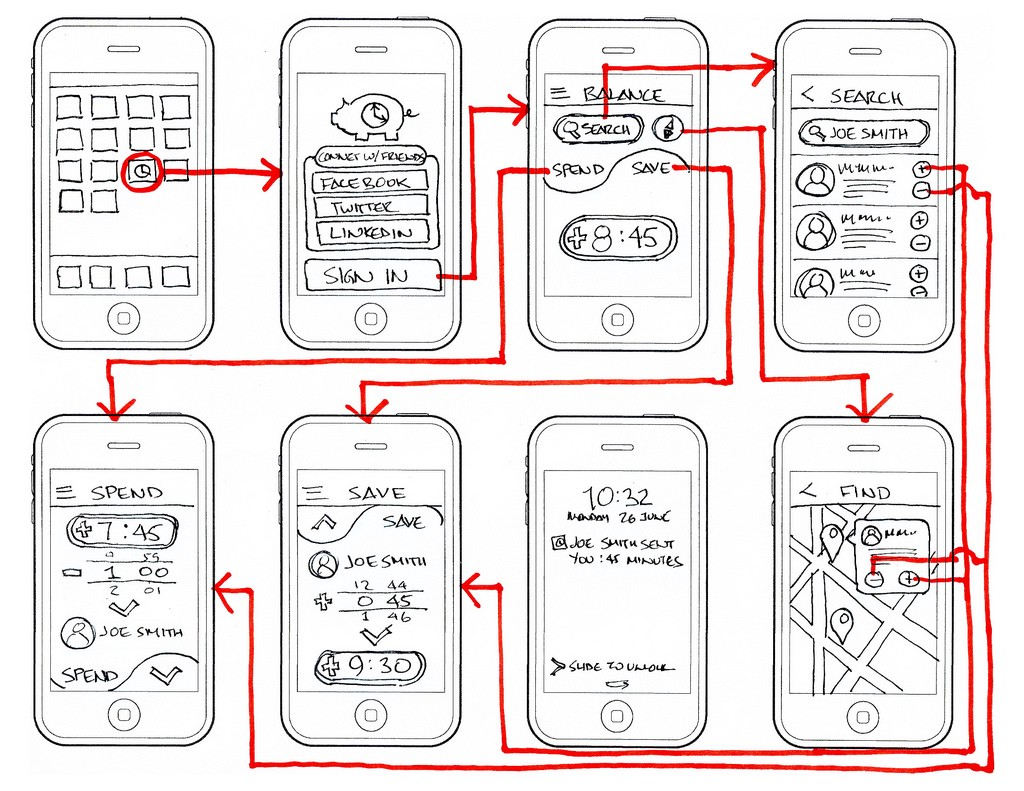
\includegraphics[width=\columnwidth]{storyboard-map}
\end{frame}


\begin{frame}{Cvičení - Use case diagram}
	\begin{itemize}
		\item zobrazuje aktéry a jejich akce (businessově)
		\begin{itemize}
			\item za jakým účelem uživatel používá aplikaci
			\item zvolit vhodnou granularitu - musí být čitelné
		\end{itemize}  
	\end{itemize}
	
	todo obrázek
	
\end{frame}


\begin{frame}{Cvičení - rozložení stránky}
	\begin{itemize}
		\item hlavička
		\item navigace
		\item obsah
		\item patka 
	\end{itemize}
\end{frame}

\begin{frame}{Cvičení - rozložení webové stránky}
  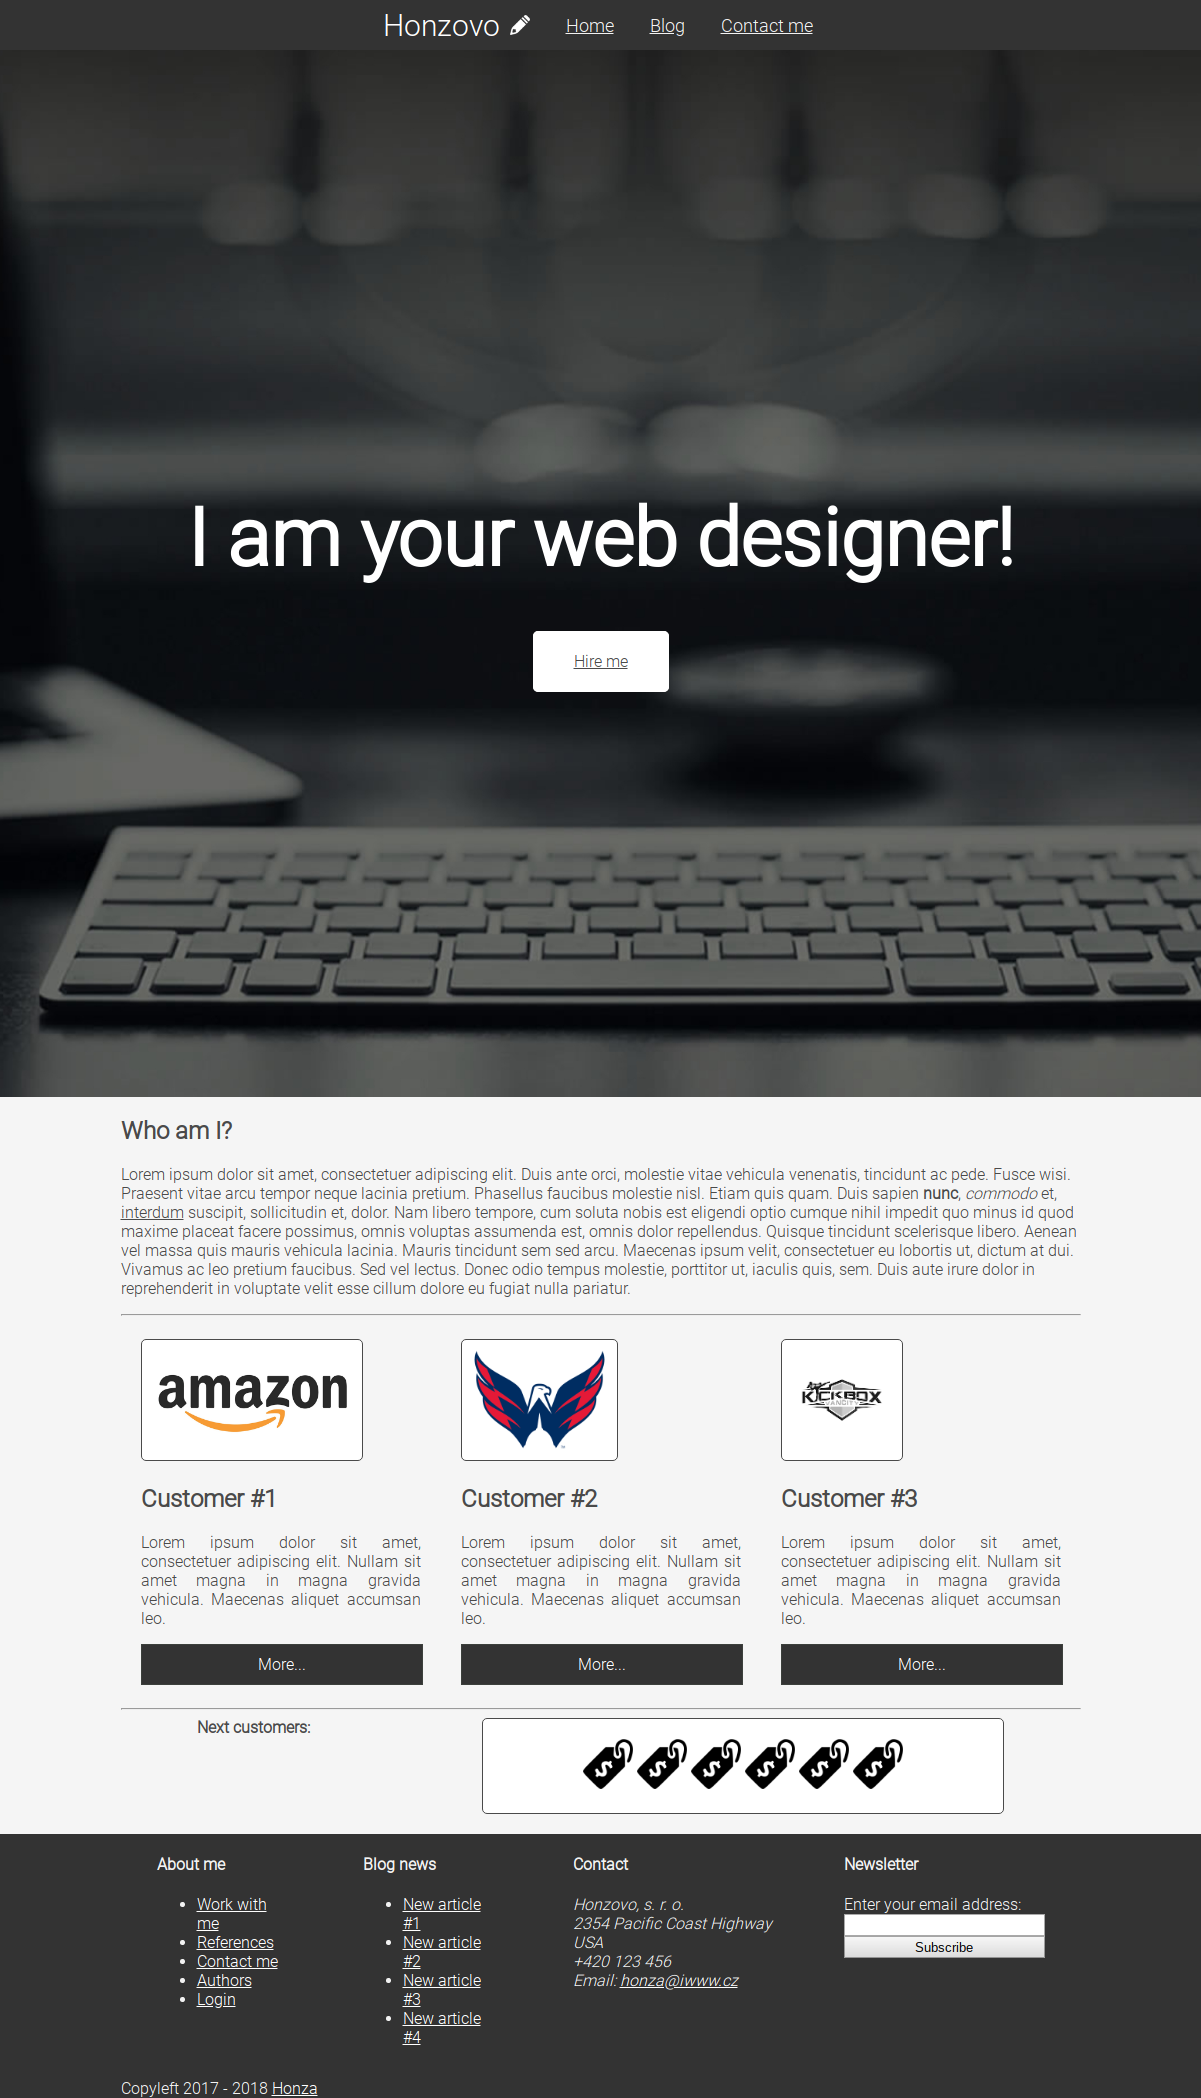
\includegraphics[scale=0.1]{project}
\end{frame}

\section{W3SCHOOLS -- HTML}

\begin{frame}[fragile, shrink=0]{Projektové cvičení -- hlavička}

\begin{lstlisting}[language=HTML5]
<!DOCTYPE html>
<html>
	<head>
		<title>Honzovo</title>
	</head>
	<body>
<header>
    <div id="header-web-title">Honzovo</div>
    <img id="header-logo" src="./images/logo.png"/>
    <nav id="nav">
        <a href="#">Home</a>
        <a href="#">Blog</a>
        <a href="#">Contact me</a>
    </nav>
</header>
\end{lstlisting}
	
\end{frame}

\begin{frame}[fragile, shrink=0]{Projektové cvičení -- hero}

\begin{lstlisting}[language=HTML5]
<section id="hero">
    <div>
        <h1>I am your web designer!</h1>
        <a href="#">
            Hire me
        </a>
    </div>
</section>
\end{lstlisting}
	
\end{frame}



\begin{frame}[fragile, shrink=0]{Projektové cvičení -- obsah I.}

\begin{lstlisting}[language=HTML5]
<main>
    <div>
    <div>
        <h2>Who am I?</h2>
        <p>
          Duis sapien <strong>nunc</strong>, 
          <i>commodo</i> et,
           <u>interdum</u> suscipi
        </p>
        <hr>

        <div>
            <div>
                <img src="/images/customerOne.jpg">
                <h2>Customer #1</h2>
                <p>Lorem ipsum.</p>
                <a href="#">
                    <div>More...</div>
                </a>
            </div>
        ...
        two more customers
       


     
        
\end{lstlisting}
	
\end{frame}

\begin{frame}[fragile, shrink=0]{Projektové cvičení -- obsah II.}

\begin{lstlisting}[language=HTML5]
<hr/>
<div >
    <strong>Next customers:</strong>
    <div>
        <img src="./images/price.png">
        <img src="./images/price.png">
    </div>
</div>
...
</...></main>
\end{lstlisting}
	
\end{frame}


\begin{frame}[fragile, shrink=0]{Projektové cvičení -- odkazy v patičce}

\begin{lstlisting}[language=HTML5]
<footer>
  <div>
     <div>
        <section>
        	<h4>About me</h4>
                <ul>
                    <li><a href="#">Work with me</a></li>
                    <li><a href="#">References</a></li>
                    <li><a href="#">Contact me</a></li>
                    <li><a href="#">Authors</a></li>
                    <li><a href="#">Login</a></li>
                </ul>
            </section>

            <section>
                <h4>Blog news</h4>
                <ol>
                    <li><a href="#">New article #1</a></li>
                    <li><a href="#">New article #2</a></li>
                    <li><a href="#">New article #3</a></li>
                    <li><a href="#">New article #4</a></li>
                </ol>
            </section>
            
\end{lstlisting}
	
\end{frame}



\begin{frame}[fragile, shrink=0]{Projektové cvičení -- adresa}

\begin{lstlisting}[language=HTML5]     
<section>
    <h4>Contact</h4>
    <address>
        Honzovo, s. r. o.<br>
        2354 Pacific Coast Highway<br>
        USA<br>
        +420 123 456<br>
        Email: <a href="mailto:honza@iwww.cz">
        honza@iwww.cz</a><br>
    </address>
</section>
\end{lstlisting}
	
\end{frame}




\begin{frame}[fragile, shrink=0]{Projektové cvičení -- newsletter form }

\begin{lstlisting}[language=HTML5]
<section id="footer-newsletter">
    <h4>Newsletter</h4>
    <form method="POST" action="#">
        <div>
            <label>
            Enter your email address: 
            </label>
        </div>
        <div>
            <input type="text" 
            name="email"/>
        </div>
        <div>
            <input type="submit" 
            name="newsletter"
             value="Subscribe">
        </div>
    </form>
</section>    
</div   
\end{lstlisting}
	
\end{frame}



\begin{frame}[fragile, shrink=0]{Projektové cvičení -- licence }

\begin{lstlisting}[language=HTML5]
        <section>
            <p>
              Copyleft
              2017 - 2018 
              <a href="https://github.com">
                Honza
              </a>
            </p>
      </section>
   </div>
</footer>

</body>
</html>
\end{lstlisting}
	
\end{frame}




\begin{frame}{Analýza webové stránky - ex post}

\begin{itemize}
	\item validátor - https://validator.w3.org/
	\item optimalizace - LightHouse
\end{itemize}
	
\end{frame}

\section{Opakování}

\begin{frame}{Dev tools -- google chrome}

	\begin{itemize}
		\item zobrazení klávesou \emph{F12}
		\item nabízí spoustu možností pro vývojáře
		\begin{itemize}
			\item inspekce jednotlivých elementů
			\item sledování síťového provozu (request, response, timing)
			\item profilování a debugování na straně klienta
			\item auditování (výkon, přístupnost, atd.)
			
		\end{itemize} 
	\end{itemize}

\end{frame}

\begin{frame}[fragile]{Základy HTML}

\begin{itemize}
	\item sémantika -- co výraz znamená

\end{itemize}
\begin{lstlisting}[language=HTML5]
<h1> Nadpis </h1>
<div id="nadpis"> Nadpis </div>
\end{lstlisting}
	
	\begin{itemize}

	\item syntaxe -- jak výraz zapsat
\end{itemize}
\begin{lstlisting}[language=HTML5]
<br />
<br></br>
\end{lstlisting}

\end{frame}

\begin{frame}{HTML5}
	  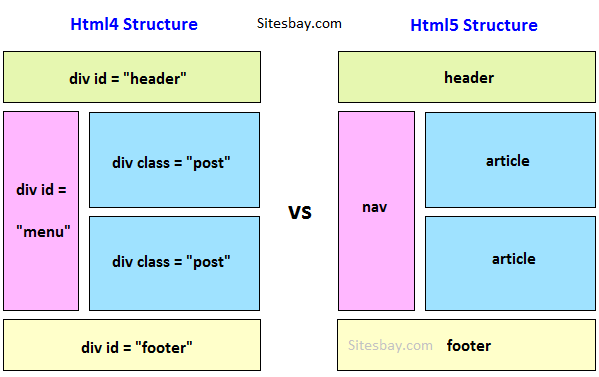
\includegraphics[width=\columnwidth]{html4-vs-html5}
\end{frame}


\begin{frame}{Prvky pro definici struktury stránky}
	\begin{itemize}
		\item header -- úvodní obsah
		\item section -- seskupení obsahu
		\item article -- článek / část obsahu (samostatný a distribuovatelný obsah)
		\item nav -- skupina navigačních odkazů
		\item aside -- část stránky, která okrajově souvisí o hlavním obsahem (postranní panel, blok reklam)
		\item footer -- zápatí obsahu 
	\end{itemize}
\end{frame}


\begin{frame}[shrink]{Opakování základních tabů tagů}
\begin{multicols}{2}

	\begin{itemize}
	\item Struktura stránky
		\begin{itemize}
			\item html
			\item head
			\item body
		\end{itemize}
	\end{itemize}

	\begin{itemize}
		\item Struktura obsahu
		\begin{itemize}
			\item section
			\item header
			\item footer
			\item nav
			\item article 
		\end{itemize}
	\end{itemize}	
	
	\begin{itemize}	
		\item Obsah
		\begin{itemize}
			\item Hx -- nadpis
			\item p -- odstavec
			\item a -- odkaz
			\item ul -- odrážkový seznam
			\item ol -- číslovaný seznam
			\item li -- položka seznamu
			\item img -- obrázek
			\item br
		\end{itemize}
	\end{itemize}

	\begin{itemize}	
		\item Formát
		\begin{itemize}
			\item strong
			\item em
			\item small
			\item code	
		\end{itemize}
	\end{itemize}
	
	\begin{itemize}	
		\item Tabulky
		\begin{itemize}
			\item table -- tabulka
			\item thead -- hlavička tabulky
			\item tbody -- tělo tabulky
			\item tfoot -- patka tabulky
			\item tr -- řádek
			\item td -- běžná buňka
			\item th -- 
		\end{itemize}
	\end{itemize}


\end{multicols}
\end{frame}


\begin{frame}{Kontrolní otázky}
\begin{itemize}
	\item Jak začnu s vytvořením webu?
	\item Jaké nástroje pro vývoj webu potřebuji?
	\item Co je to hosting?
	\item Jaký je rozdíl mezi sémantikou a syntaxí?
	\item Jak vypadá základní kostra HTML?
	\item Co je to HTML a k čemu slouží?
	\item Co je to CSS a k čemu slouží?
\end{itemize}
	
\end{frame}


	  

\end{document}